\documentclass[11pt]{article}

\usepackage[margin=1in]{geometry}
\usepackage{amsmath, amssymb, amsfonts}
\usepackage{bm}
\usepackage{graphicx}
\usepackage{enumitem}
\usepackage{tikz}
\usetikzlibrary{calc}
\usepackage[most]{tcolorbox}
\usepackage{hyperref}
\usepackage{booktabs}
\usepackage[numbers]{natbib}

\title{Ice Rheology: Creep Mechanisms and Glen's Flow Law}
\author{Brent Minchew \\Caltech Ge 193, Spring 2026}
\date{}

\begin{document}

\maketitle

%===================================================================
% Topics Covered
%===================================================================
\section*{Topics Covered}

\begin{itemize}
  \item The four creep mechanisms in polycrystalline ice
  \item The composite flow law of Goldsby \& Kohlstedt (2001)
  \item How the composite flow law reduces to Glen's flow law
  \item Physical basis for the rate factor $A$ and the creep exponent $n$
\end{itemize}

\noindent\textbf{Primary reference:} Cuffey \& Paterson, \textit{Physics of Glaciers}, 4th ed., Chapter~3; Goldsby \& Kohlstedt (2001).

%===================================================================
% SECTION 1 -- Introduction and Motivation
%===================================================================
\section{Introduction and Motivation}

In the preceding lectures, we stated Glen's flow law as the constitutive relation for glacier ice:
\begin{equation}
  \dot{\varepsilon}_{ij} = A\,\tau_e^{\,n-1}\,\tau_{ij},
  \label{eq:glen_recap}
\end{equation}
with $n = 3$ the typical assumption and $A$ a temperature-dependent rate factor.  We used this relation to derive velocity profiles, build the SIA, formulate the full Stokes system, and study the SSA equations.  Throughout, we treated $A$ and $n$ as given without examining their physical basis.

\medskip
\noindent The goal of this lecture is to understand where Eq.~\ref{eq:glen_recap} comes from.  
\medskip

\noindent Ice is a polycrystalline material, and its deformation is governed by several grain-scale mechanisms that operate in parallel or in series depending on the stress, temperature, and grain size.  A grain is a single crystal and the terms `grain' and `crystal' are often casually interchanged. Polycrystalline simply means there are many grains. Understanding the deformation mechanisms is important for at least three reasons:
\begin{enumerate}
  \item It reveals when Glen's law is a good approximation and when it breaks down.
  \item It explains the temperature dependence of the rate factor $A$ through activation energies.
  \item It clarifies the physical meaning of the creep exponent $n$ and why the commonly assumed value of $n = 3$ is not a material property but rather a special case that, unfortunately for the field, was casually taken to be general several decades ago. The near-universal assumption of $n=3$ has severely limited progress in glacier dynamics, as will no doubt become increasingly clear in the coming years and decades. 
\end{enumerate}

\medskip
\noindent\textbf{Plan for this lecture.}  We first review the general form of creep flow laws for crystalline materials (\S\ref{sec:general_form}).  We then discuss the four creep mechanisms identified in ice (\S\ref{sec:creep_mechanisms}).  Next, we present the composite flow law that combines all four mechanisms (\S\ref{sec:composite}).  Finally, we show how this composite law reduces to Glen's flow law under the conditions typically assumed in glaciology (\S\ref{sec:glen_reduction}).

%===================================================================
% SECTION 2 -- General Form of Creep Flow Laws
%===================================================================
\section{General Form of Creep Flow Laws}
\label{sec:general_form}

Rheological data for crystalline materials are typically analyzed with a power law of the form
\begin{equation}
  \boxed{\dot{\varepsilon}_e = A_0 \,\frac{\tau_e^{\,n}}{d^r} \,\exp\!\left(-\frac{Q + pV}{RT}\right),}
  \label{eq:general_creep}
\end{equation}
where:
\begin{itemize}
  \item $\dot{\varepsilon}_e$ is the effective strain rate and $\tau_e$ is the effective deviatoric stress,
  \item $A_0$ is a material-dependent prefactor,
  \item $n$ is the stress exponent,
  \item $d$ is the mean grain size and $r$ is the grain-size exponent,
  \item $Q$ is the activation energy for creep,
  \item $p$ is the pressure and $V$ is the activation volume,
  \item $R$ is the gas constant and $T$ is the absolute temperature.
\end{itemize}

\noindent The values of $n$, $r$, and $Q$ are diagnostic: they identify which physical mechanism controls the creep rate.  For example, a stress exponent $n = 1$ indicates diffusion-controlled flow, while $n > 1$ indicates a dislocation-mediated process.  A grain-size exponent $r > 0$ indicates that grain boundaries participate in the rate-limiting process.

\medskip
\noindent The activation volume $V$ describes the pressure dependence of the creep rate.  For ice, $V \approx -13 \times 10^{-6}$~m$^3$\,mol$^{-1}$ \cite{GoldsbyKohlstedt2001}.  The $pV$ term modifies the effective activation energy under pressure: at the base of a 3~km-thick ice sheet, $p \approx \rho_i g h \approx 27$~MPa, giving $pV \approx -0.35$~kJ\,mol$^{-1}$, which is negligible compared to $Q \approx 60$~kJ\,mol$^{-1}$.  The activation volume is therefore typically omitted in glaciological applications, reducing the Arrhenius factor to $\exp(-Q/RT)$.

%===================================================================
% SECTION 3 -- The Four Creep Mechanisms
%===================================================================
\section{The Four Creep Mechanisms in Ice}
\label{sec:creep_mechanisms}

Laboratory experiments on fine-grained ice by \cite{GoldsbyKohlstedt2001} reveal four distinct creep regimes, each characterized by different values of $n$ and $r$.  The stress exponents and other parameters reported below are laboratory values, determined from experiments on small ($\sim$cm-scale), initially isotropic samples with controlled grain sizes.  As discussed below, whether these values apply quantitatively to natural glacier ice---which develops crystal-orientation fabric, contains impurities and interstitial water, and has grain sizes that evolve with deformation---remains an active area of research.  The physical mechanisms themselves, however, are well established.  A useful organizing principle is to distinguish between \textbf{intragranular} deformation mechanisms and \textbf{intergranular} accommodation mechanisms:
\begin{itemize}
  \item \textbf{Intragranular} mechanisms deform the interior of individual grains.  In ice, these are dislocation creep (the motion of dislocations through the crystal lattice) and diffusion (the transport of molecules through the lattice or along grain boundaries driven by stress gradients).  These are the fundamental crystalline deformation mechanisms---they produce strain.
  \item \textbf{Intergranular} accommodation mechanisms operate at grain boundaries to maintain compatibility between neighboring grains.  The most important is grain boundary sliding (GBS), in which neighboring grains translate and rotate relative to one another along their shared boundary.
\end{itemize}

\noindent A single crystal deforming in isolation needs only intragranular mechanisms.  In a polycrystal, however, grains must deform compatibly with their neighbors---each grain is constrained by the grains surrounding it.  This compatibility requirement means that the intragranular deformation mechanisms must be accompanied by an accommodation mechanism that resolves the mismatch at grain boundaries.  Accommodation can be achieved either intragranularly (by activating hard slip systems within each grain, as in dislocation creep) or intergranularly (by GBS).  The nature of this coupling---which mechanism is rate-limiting---determines the observed creep parameters.

\medskip
\noindent The four creep regimes identified by \cite{GoldsbyKohlstedt2001} are, in order of decreasing stress: dislocation creep, GBS-accommodated basal slip (``superplastic flow''), basal-slip-accommodated GBS, and diffusional flow.  Each is described by a flow law of the form given in equation~\eqref{eq:general_creep}.  We discuss each mechanism below.

% CHALKBOARD DRAWING 1:
% Sketch a schematic log(strain rate) vs. log(stress) plot showing four creep regimes
% with different slopes, similar to Figure 5 of Goldsby & Kohlstedt (2001).

\subsection{Dislocation Creep ($n = 4.0$, $r = 0$)}
\label{sec:dislocation}

At the highest stresses, deformation is controlled by the motion of dislocations through the crystal lattice---a purely intragranular process.  Dislocations are line defects in the crystal structure, and their motion under an applied stress produces macroscopic strain.  In ice, the dominant slip system is the basal plane (the hexagonal plane perpendicular to the $c$-axis), on which dislocations glide easily.  Non-basal slip (on prismatic and pyramidal planes) is much more difficult---single crystals oriented for easy basal slip can deform $>10^5$ times faster than those oriented for hard slip.

\medskip
\noindent Dislocation creep in polycrystalline ice is characterized by:
\begin{itemize}
  \item A stress exponent $n \approx 4.0$, measured in experiments at high confining pressure.  This value is consistent across several independent studies, though uncertainties of $\pm 0.5$ are typical for laboratory fits.
  \item No grain-size dependence ($r = 0$): the strain rate depends only on stress and temperature, because the rate-limiting step is dislocation motion within grains.
  \item An activation energy $Q \approx 60$~kJ\,mol$^{-1}$ below $\sim$258~K, increasing to $\sim$180~kJ\,mol$^{-1}$ above 258~K due to premelting at grain boundaries.
\end{itemize}

\noindent The rate-limiting step in dislocation creep is dislocation climb, in which edge dislocations move perpendicular to their glide plane by absorbing or emitting point defects.  Climb allows dislocations to bypass obstacles (other dislocations, grain boundaries), and is controlled by volume self-diffusion.  The equivalence of the activation energy for dislocation creep ($\sim$60~kJ\,mol$^{-1}$) with that for volume self-diffusion of hydrogen and oxygen in ice confirms that climb limits the creep rate.

\medskip
\noindent The creep strength of polycrystalline ice in the dislocation creep regime is intermediate between the strengths of single crystals oriented for easy (basal) and hard (non-basal) slip.  This reflects the fact that each grain in a polycrystal must deform compatibly with its neighbors, requiring activation of both basal and non-basal slip systems.  In this regime, the intergranular accommodation is achieved entirely by intragranular means---hard (non-basal) slip within each grain resolves the mismatch at grain boundaries, so GBS plays no role and $r = 0$.

\subsection{GBS-Accommodated Basal Slip --- Superplastic Flow ($n = 1.8$, $r = 1.4$)}
\label{sec:superplastic}

At intermediate stresses, a transition occurs to a creep regime characterized by $n \approx 1.8$ and a strong dependence on grain size ($r \approx 1.4$).  In this regime, the intragranular mechanism is basal slip (easy glide on the basal plane), while the intergranular accommodation mechanism is grain boundary sliding (GBS).

\medskip
\noindent Recall that in dislocation creep, grain-to-grain compatibility is achieved by an intragranular process: activation of hard (non-basal) slip systems within each grain.  In the superplastic regime, an intergranular process takes over this role: grains slide past one another along their boundaries, accommodating the mismatch produced by easy basal slip within each grain.  Because GBS is the slower of the two serial processes (basal slip and GBS) under these conditions, GBS limits the overall strain rate.

\begin{tcolorbox}[
  colback=blue!5,
  colframe=blue!50!black,
  title={\textbf{Key point: serial vs.\ parallel processes}}
]
When two deformation processes operate in \textbf{series} (both must occur for macroscopic strain), the slower process limits the rate:
\begin{equation}
  \dot{\varepsilon}_{\text{total}}^{-1} = \dot{\varepsilon}_{\text{basal}}^{-1} + \dot{\varepsilon}_{\text{GBS}}^{-1}.
\end{equation}
When two processes operate in \textbf{parallel} (either alone can produce macroscopic strain), their rates add:
\begin{equation}
  \dot{\varepsilon}_{\text{total}} = \dot{\varepsilon}_1 + \dot{\varepsilon}_2.
\end{equation}
Basal slip (intragranular) and GBS (intergranular) are serial processes: basal slip produces strain within grains, but without GBS to accommodate grain-to-grain incompatibility, the polycrystal cannot deform.  The transition from dislocation creep ($n = 4$) to superplastic flow ($n = 1.8$) occurs when GBS becomes slower than the hard-slip accommodation mechanism and thereby becomes the rate-limiting step.  This is a transition in the intergranular accommodation mechanism---from hard slip within grains to sliding between grains.
\end{tcolorbox}

\noindent The superplastic regime is characterized by:
\begin{itemize}
  \item A stress exponent $n \approx 1.8$.
  \item A grain-size exponent $r \approx 1.4$: finer-grained ice deforms faster because there is more grain-boundary area per unit volume.
  \item An activation energy $Q \approx 49$~kJ\,mol$^{-1}$ below $\sim$258~K, increasing at higher temperatures due to premelting.
\end{itemize}

\noindent Microstructural evidence supports the role of GBS in this regime.  Samples deformed in the $n = 1.8$ regime show minimal grain flattening (unlike dislocation creep, where grains are substantially deformed), numerous four-grain junctions (a signature of grain switching associated with GBS), and straight, regular grain boundaries (unlike the irregular boundaries produced by dynamic recrystallization in dislocation creep).

\subsection{Basal-Slip-Accommodated GBS ($n = 2.4$, $r = 0$)}
\label{sec:basal_slip}

At still lower stresses and for the finest grain sizes ($d \lesssim 5$~$\mu$m), a third creep regime appears with $n = 2.4$ and no grain-size dependence ($r = 0$).  Here, the intergranular mechanism (GBS) is faster than the intragranular mechanism (basal slip), so basal slip becomes the rate-limiting step.

\medskip
\noindent This represents the other limit of the serial intragranular/intergranular process.  In the superplastic regime ($n = 1.8$), the intergranular process (GBS) is slower and controls the rate.  At lower stresses, the strain-rate contributions cross over because of their different stress exponents, and now the intragranular process (basal slip) is the slower of the two.  Because the rate-limiting step is intragranular, the creep rate is independent of grain size ($r = 0$).

\medskip
\noindent The creep parameters in this regime---$n = 2.4$ and $Q \approx 60$~kJ\,mol$^{-1}$---are in excellent agreement with those for basal slip in single crystals, confirming that basal slip is rate-limiting.  The absolute creep strengths of polycrystalline samples in this regime also agree well with single-crystal basal-slip data.  This regime has only been observed experimentally for very fine-grained samples ($d \lesssim 5$~$\mu$m) at very low stresses and is likely inaccessible for the grain sizes relevant to glacier flow.

\subsection{Diffusional Flow ($n = 1.0$, $r = 2$--$3$)}
\label{sec:diffusion}

At the lowest stresses, deformation can in principle occur by diffusion of molecules either through the crystal lattice (Nabarro--Herring creep, $r = 2$) or along grain boundaries (Coble creep, $r = 3$).  Both are intragranular deformation mechanisms---they produce strain by rearranging molecules within or between grains in response to stress gradients.  The grain-size dependence ($r > 0$) arises because smaller grains have shorter diffusion paths, not because diffusion is an accommodation mechanism.  Both are characterized by a stress exponent $n = 1$ (Newtonian behavior).

\medskip
\noindent The diffusional flow rate for polycrystalline ice can be written as
\begin{equation}
  \dot{\varepsilon}_{\text{diff}} = \frac{42\,\tau_e\,V_m}{R\,T\,d^2}\!\left(D_v + \frac{\pi\,\delta}{d}\,D_b\right),
  \label{eq:diffusion}
\end{equation}
where $V_m$ is the molar volume, $D_v$ is the volume diffusion coefficient, $\delta$ is the grain-boundary width, and $D_b$ is the grain-boundary diffusion coefficient.

\medskip
\noindent Based on estimates of the diffusion parameters for ice, \cite{GoldsbyKohlstedt2001} conclude that diffusional flow is unattainably slow at laboratory strain rates for grain sizes $\gtrsim 3$~$\mu$m.  For glaciologically relevant grain sizes (typically $\geq 1$~mm), the diffusional flow rate is negligible compared to the other creep mechanisms.  Diffusional flow has not been observed experimentally in ice even for samples with grain sizes as small as 3~$\mu$m.

\begin{tcolorbox}[
  colback=blue!5,
  colframe=blue!50!black,
  title={\textbf{Key point: the dominant creep mechanism depends on conditions}}
]
The four creep mechanisms are summarized below with their laboratory-derived parameters.  At glaciologically relevant conditions (shear stresses $\lesssim 0.1$~MPa, grain sizes $\geq 1$~mm, temperatures 233--273~K), the composite flow law suggests that the superplastic flow regime ($n \approx 1.8$) is the rate-limiting mechanism for much of the stress range encountered in glaciers and ice sheets.

\medskip
\begin{center}
\small
\begin{tabular}{lccccl}
\toprule
\textbf{Mechanism} & $n$ & $r$ & $Q$ (kJ\,mol$^{-1}$) & \textbf{Scale} & \textbf{Rate-limiting step} \\
\midrule
Dislocation creep & 4.0 & 0 & 60 & Intra & Dislocation climb \\
GBS-accomm.\ basal slip & 1.8 & 1.4 & 49 & Inter & Grain boundary sliding \\
Basal-slip-accomm.\ GBS & 2.4 & 0 & 60 & Intra & Basal slip \\
Diffusional flow & 1.0 & 2--3 & $\sim$60 & Intra & Vol./boundary diffusion \\
\bottomrule
\end{tabular}
\end{center}
\end{tcolorbox}

%===================================================================
% SECTION 4 -- The Composite Flow Law
%===================================================================
\section{The Composite Flow Law}
\label{sec:composite}

The flow of polycrystalline ice cannot be adequately described by a single power law (i.e., Glen's Flow Law) with one set of creep parameters.  \cite{GoldsbyKohlstedt2001} proposed a composite constitutive equation that combines all four creep mechanisms:
\begin{equation}
  \boxed{\dot{\varepsilon}_e = \dot{\varepsilon}_{\text{diff}} + \left(\frac{1}{\dot{\varepsilon}_{\text{basal}}} + \frac{1}{\dot{\varepsilon}_{\text{gbs}}}\right)^{-1} + \dot{\varepsilon}_{\text{disl}},}
  \label{eq:composite}
\end{equation}
where $\dot{\varepsilon}_{\text{diff}}$ is the diffusional flow rate, $\dot{\varepsilon}_{\text{basal}}$ is the basal-slip rate, $\dot{\varepsilon}_{\text{gbs}}$ is the GBS rate, and $\dot{\varepsilon}_{\text{disl}}$ is the dislocation creep rate. It can be shown that this is the minimum viable representation for viscous (creep) deformation in isotropic ice Ih (all ice we're interested in on Earth is ice Ih). 

\medskip
\noindent The structure of equation~\eqref{eq:composite} reflects the physical relationships between intragranular and intergranular processes:
\begin{itemize}
  \item \textbf{Basal slip (intragranular) and GBS (intergranular) are in series} (the harmonic mean): both must operate for grain-size-sensitive deformation, and the slower process limits the rate.  At high stresses, the intergranular process (GBS) is slower and the effective stress exponent approaches $n = 1.8$; at low stresses, the intragranular process (basal slip) is slower and $n \to 2.4$.
  \item \textbf{Dislocation creep (intragranular) operates in parallel} with the grain-size-sensitive mechanisms: it provides an independent intragranular deformation pathway through the activation of multiple slip systems, with hard slip serving as the intergranular accommodation mechanism.  At high stresses, dislocation creep dominates because of its high stress exponent ($n = 4$).
  \item \textbf{Diffusional flow also operates in parallel}: it provides yet another independent intragranular deformation pathway, dominant only at very low stresses and very small grain sizes.
\end{itemize}

\noindent Each term in equation~\eqref{eq:composite} has the form of equation~\eqref{eq:general_creep}, with parameters given in Table~\ref{tab:parameters}.

\begin{table}[ht]
\centering
\caption{Constitutive equation parameters from \cite{GoldsbyKohlstedt2001}.  Two sets of parameters are given for dislocation creep and GBS-accommodated basal slip to account for the increase in activation energy above $\sim$258~K due to premelting.}
\label{tab:parameters}
\begin{tabular}{lcccc}
\toprule
\textbf{Creep regime} & $A_0$ (units vary) & $n$ & $r$ & $Q$ (kJ\,mol$^{-1}$) \\
\midrule
Dislocation creep ($T < 258$~K) & $4.0 \times 10^5$~MPa$^{-4.0}$\,s$^{-1}$ & 4.0 & 0 & 60 \\
Dislocation creep ($T > 258$~K) & $6.0 \times 10^{28}$~MPa$^{-4.0}$\,s$^{-1}$ & 4.0 & 0 & $\sim$181 \\
GBS-accomm.\ basal slip ($T < 255$~K) & $3.9 \times 10^{-3}$~MPa$^{-1.8}$\,m$^{1.4}$\,s$^{-1}$ & 1.8 & 1.4 & 49 \\
GBS-accomm.\ basal slip ($T > 255$~K) & $3.0 \times 10^{26}$~MPa$^{-1.8}$\,m$^{1.4}$\,s$^{-1}$ & 1.8 & 1.4 & $\sim$192 \\
Basal-slip-accomm.\ GBS & $5.5 \times 10^{7}$~MPa$^{-2.4}$\,s$^{-1}$ & 2.4 & 0 & 60 \\
\bottomrule
\end{tabular}
\end{table}

\noindent Predictions of this composite flow law agree well with published laboratory creep data for coarse-grained ($d \geq 1$~mm) polycrystalline ice across a wide range of temperatures and stresses.

\medskip
\noindent\textbf{A caveat on laboratory-to-field scaling.}  The parameters in Table~\ref{tab:parameters} were determined from experiments on small, initially isotropic samples of pure or nearly pure ice.  Natural glacier ice differs in ways that could modify the quantitative values: it develops crystal-orientation fabric (anisotropy) during deformation, contains impurities and dust that affect grain-boundary mobility, may have interstitial water at grain boundaries (especially near the melting point), and has grain sizes that evolve with strain, temperature, and impurity content.  Scaling laboratory flow laws to ice sheets therefore introduces uncertainty in the prefactors $A_0$ and potentially in the stress exponents themselves.  The qualitative structure of the composite flow law---the existence of competing mechanisms with different stress sensitivities, and the transitions between them---is robust.  The specific numerical values (e.g., $n = 4.0$ vs.\ 3.5 for dislocation creep, or $n = 1.8$ vs.\ 2.0 for GBS) should be understood as laboratory best estimates, not exact constants of nature.  Throughout this lecture, we use the \cite{GoldsbyKohlstedt2001} values as a well-characterized reference point.

%===================================================================
% SECTION 5 -- Deformation Mechanism Maps
%===================================================================
\section{Deformation Mechanism Maps}
\label{sec:mechanism_maps}

The composite flow law involves multiple mechanisms with different dependencies on stress, temperature, and grain size.  A \textbf{deformation mechanism map} is a graphical tool that shows which mechanism dominates at each point in parameter space.  These maps are widely used in materials science and provide an intuitive picture of the rheological behavior of a material across a range of conditions.

\subsection{Strain Rate vs.\ Stress}

The most direct view of the composite flow law is a log-log plot of $\dot{\varepsilon}_e$ vs.\ $\tau_e$ at fixed temperature and grain size (Figure~\ref{fig:strain_rate_stress}).  At high stresses, the composite curve follows the dislocation creep line (slope $= 4$).  At lower stresses, it transitions to the GBS-accommodated basal slip line (slope $= 1.8$).  Glen's original experiments were conducted in the transition region between these two regimes, where the apparent slope is $\sim$3.

\begin{figure}[ht]
  \centering
  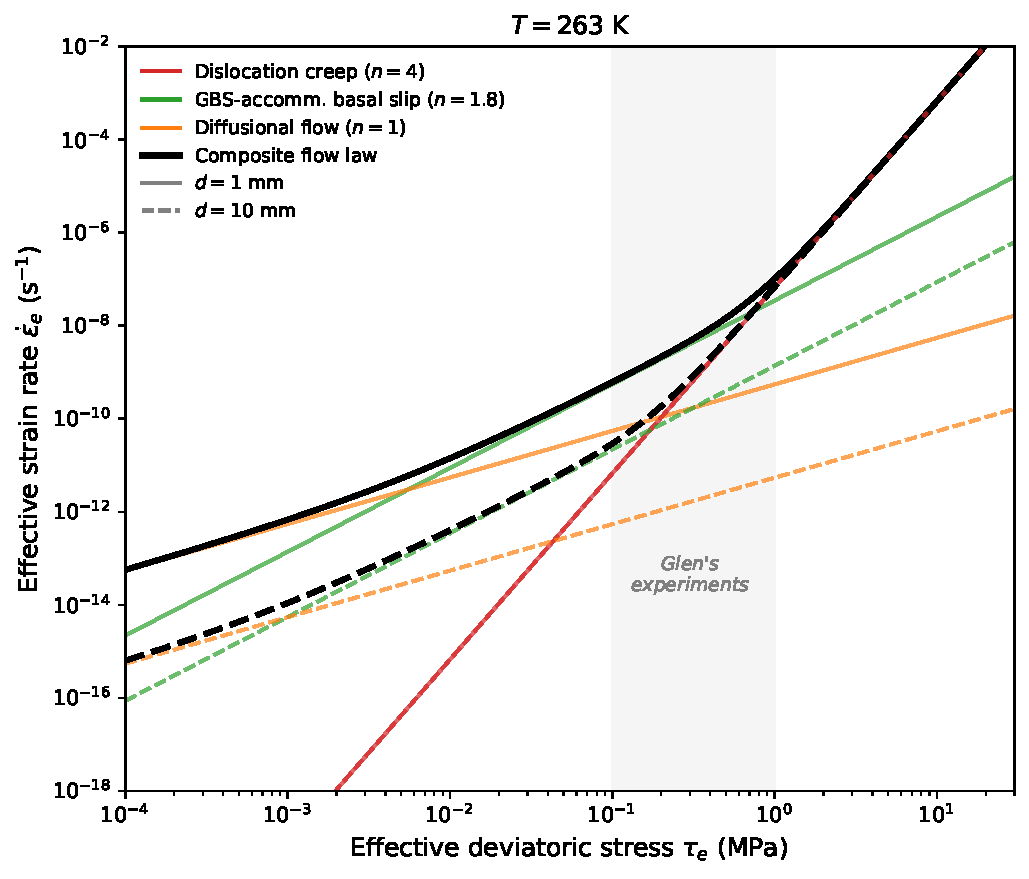
\includegraphics[width=0.75\textwidth]{figures/fig01_strain_rate_vs_stress.pdf}
  \caption{Log-log plot of effective strain rate vs.\ effective deviatoric stress at $T = 263$~K for two grain sizes: $d = 1$~mm (solid lines) and $d = 10$~mm (dashed lines).  Colors indicate the creep mechanism; black curves show the composite flow law.  Dislocation creep (red) is grain-size independent, so the solid and dashed red lines overlap.  GBS-accommodated basal slip (green) and diffusional flow (orange) are grain-size sensitive: their rates decrease for larger grains.  The crossover stress between GBS-dominated and dislocation-dominated flow shifts to lower values for larger grains.  Glen's experimental stress range (0.1--1~MPa, shaded) straddles this transition.}
  \label{fig:strain_rate_stress}
\end{figure}

\subsection{Stress--Temperature Map}

At fixed grain size, we can color the $\tau_e$--$T$ plane by the dominant mechanism (Figure~\ref{fig:mechanism_map_tau_T}).  For stresses above $\sim$1~MPa, dislocation creep dominates at all temperatures.  Below $\sim$0.1~MPa, superplastic flow dominates.  The boundary between these regimes is the locus of the crossover stress $\tau_e^*$ discussed in \S\ref{sec:glen_reduction}, and it shifts with temperature because the two mechanisms have different activation energies.

\begin{figure}[ht]
  \centering
  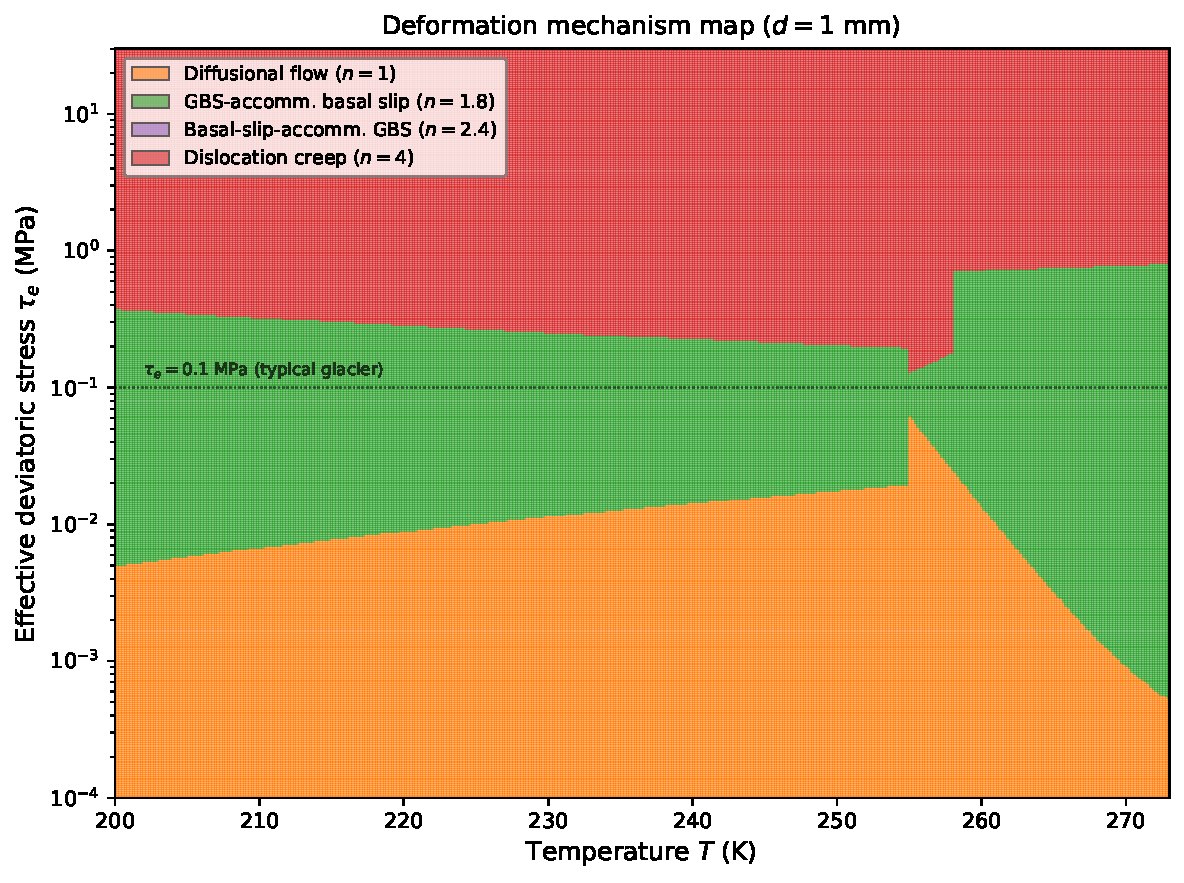
\includegraphics[width=0.75\textwidth]{figures/fig02_mechanism_map_stress_temp.pdf}
  \caption{Deformation mechanism map in $\tau_e$--$T$ space for $d = 1$~mm.  Colors indicate the dominant creep mechanism.  The dashed line marks $\tau_e = 0.1$~MPa, a typical stress scale for glaciers.  At glaciological stresses, superplastic flow ($n = 1.8$) dominates at low temperatures, while dislocation creep ($n = 4$) can become important near the melting point due to the increase in activation energy.}
  \label{fig:mechanism_map_tau_T}
\end{figure}

\subsection{Stress--Grain Size Map}

At fixed temperature, the $\tau_e$--$d$ map (Figure~\ref{fig:mechanism_map_tau_d}) reveals the role of grain size.  For large grains ($d \gtrsim 10$~mm), the grain-size-sensitive mechanisms (GBS-accommodated basal slip) require each grain boundary to accommodate more slip, reducing the GBS strain rate and expanding the domain of dislocation creep to lower stresses.  For small grains ($d \lesssim 1$~mm), the transition stress $\tau_e^*$ shifts upward and superplastic flow dominates over a wider stress range.

\begin{figure}[ht]
  \centering
  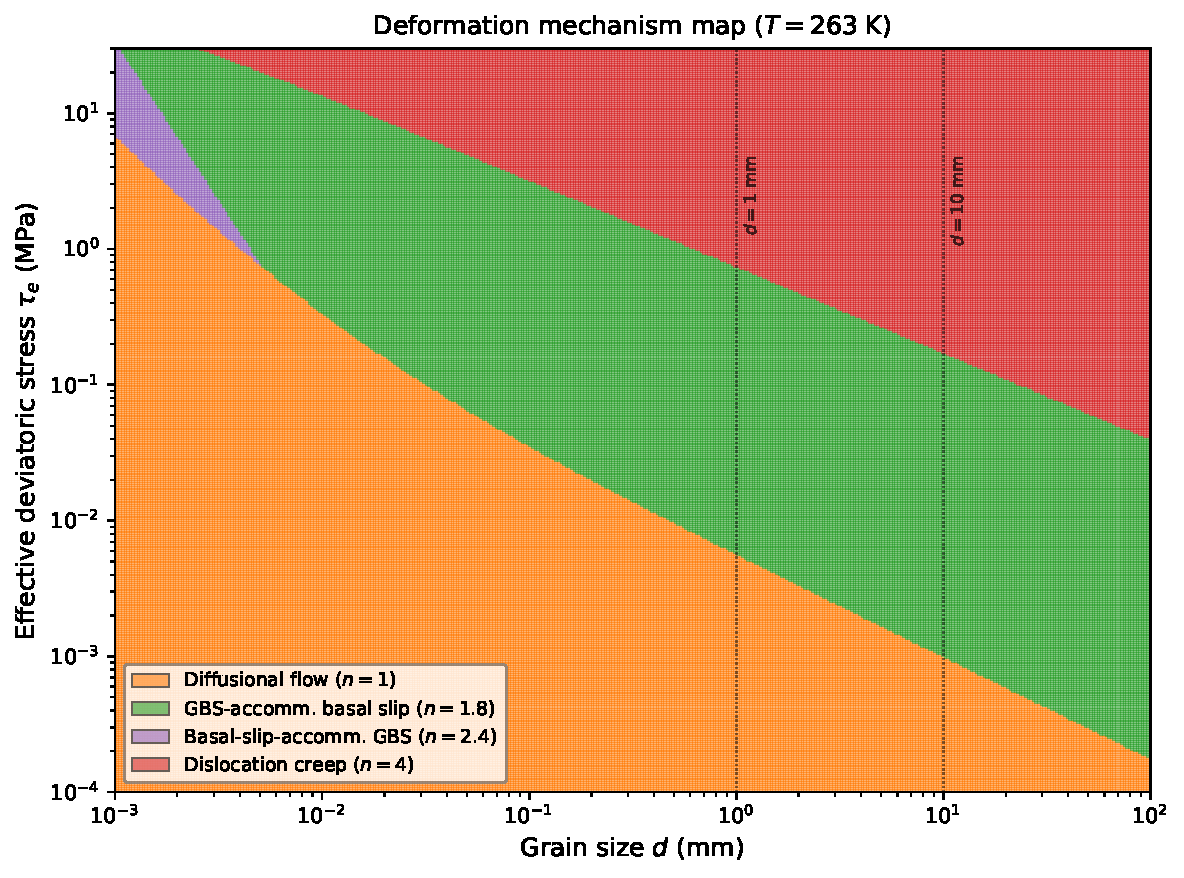
\includegraphics[width=0.75\textwidth]{figures/fig03_mechanism_map_stress_grain.pdf}
  \caption{Deformation mechanism map in $\tau_e$--$d$ space for $T = 263$~K.  Vertical lines mark $d = 1$~mm and $d = 10$~mm, spanning the range typical of glacier ice.  Finer-grained ice (e.g., ice-age ice with high impurity content) has a broader superplastic flow domain.}
  \label{fig:mechanism_map_tau_d}
\end{figure}

\subsection{The Effective Stress Exponent}

A useful complement to the mechanism map is a plot of the effective stress exponent $n_{\text{eff}}$ as a function of stress (Figure~\ref{fig:n_eff}).  This makes concrete the idea that $n = 3$ is not a fundamental value but a transitional one.

\begin{figure}[ht]
  \centering
  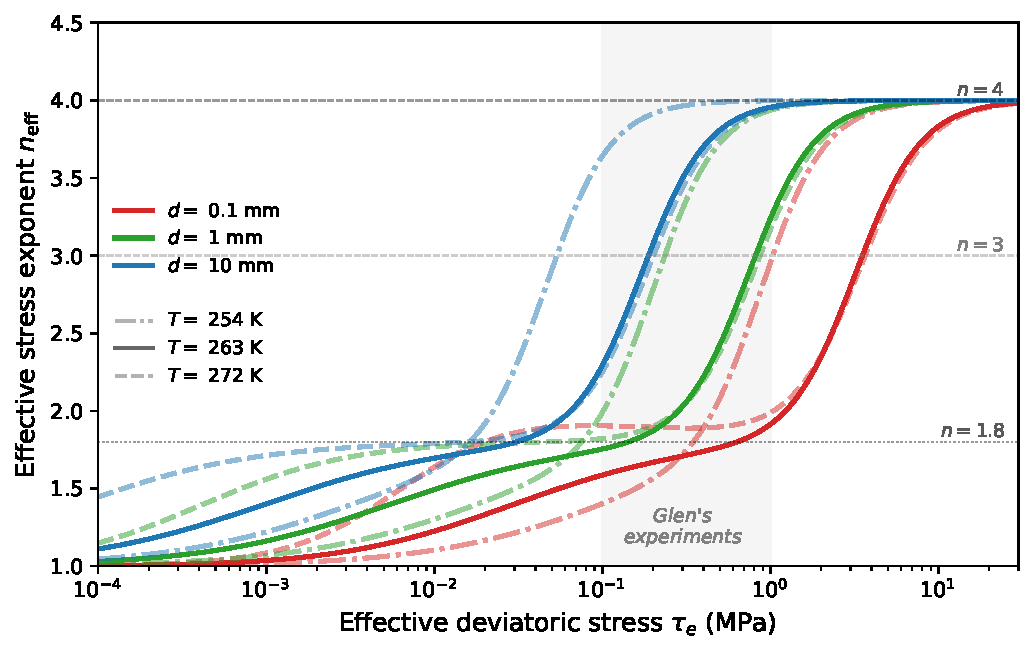
\includegraphics[width=0.75\textwidth]{figures/fig04_effective_n_vs_stress.pdf}
  \caption{Effective stress exponent $n_{\text{eff}} = \partial\log\dot{\varepsilon}_e/\partial\log\tau_e$ as a function of stress for three grain sizes---$d = 0.1$~mm (red), 1~mm (green), 10~mm (blue)---and three temperatures---$T = 254$~K (dash-dot), 263~K (solid), 272~K (dashed).  All curves transition from $n \approx 1.8$ at low stresses to $n \approx 4$ at high stresses.  The crossover stress shifts to higher values for finer grains (more grain-boundary area makes GBS more efficient) and to lower values at warmer temperatures (the higher activation energy for dislocation creep above $\sim$258~K increases $\dot{\varepsilon}_{\text{disl}}$ faster than $\dot{\varepsilon}_{\text{gbs}}$).  Glen's experimental stress range (0.1--1~MPa, shaded) sits in the transition zone for typical glacier grain sizes and near-melting temperatures.}
  \label{fig:n_eff}
\end{figure}

\noindent A striking feature of Figure~\ref{fig:n_eff} is that the crossover between GBS-accommodated basal slip and dislocation creep occurs at effective stresses of order $\sim$0.1~MPa---precisely the stress scale typical of glaciers and ice sheets.  We argue below (Example~3, \S\ref{sec:example_attractor}) that this is not a coincidence.  There is a negative feedback between the creep mechanism, the effective viscosity, and the resulting stress state.  Below the crossover, ice is relatively stiff ($n = 1.8$, weakly shear-thinning): a glacier can sustain a thick column, and thickness builds until the stress rises toward the crossover.  Above the crossover, ice softens rapidly ($n = 4$, strongly shear-thinning): the glacier flows fast and thins, reducing the stress back toward the crossover.  The crossover stress thus acts as an attractor for the stress state of the glacier.  We develop this argument quantitatively in Example~3 (\S\ref{sec:example_attractor}).

\subsection{Effect of Grain Size on the Composite Flow Law}

Figure~\ref{fig:grain_size_effect} shows the composite flow law for several grain sizes at fixed temperature.  At high stresses, all curves converge to the dislocation creep line (which is grain-size independent).  At lower stresses, finer-grained ice deforms faster because the GBS-accommodated basal slip mechanism ($r = 1.4$) is more efficient.  The crossover stress between dislocation-dominated and GBS-dominated flow shifts to higher values for finer grains.

\begin{figure}[ht]
  \centering
  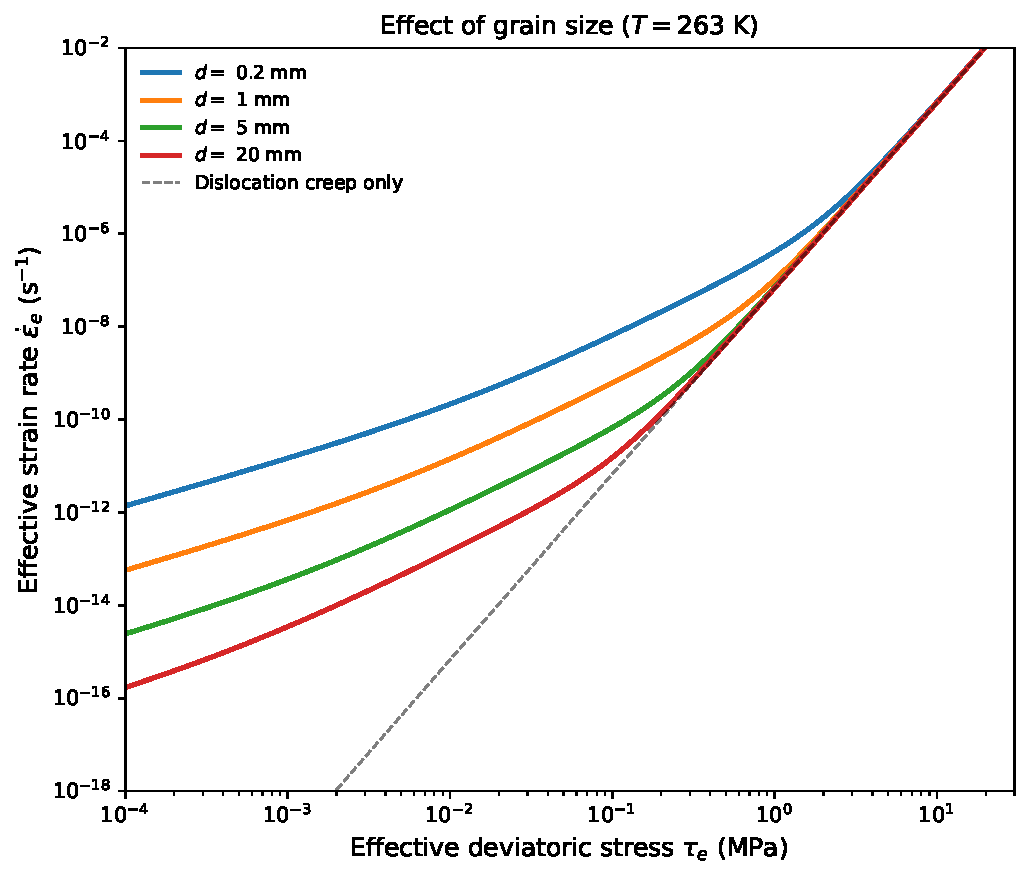
\includegraphics[width=0.75\textwidth]{figures/fig05_grain_size_effect.pdf}
  \caption{Composite flow law for different grain sizes at $T = 263$~K.  At high stresses, all curves converge to the grain-size-independent dislocation creep line (dashed).  At low stresses, finer-grained ice deforms faster due to the grain-size sensitivity of GBS-accommodated basal slip.}
  \label{fig:grain_size_effect}
\end{figure}

%===================================================================
% SECTION 6 -- Reduction to Glen's Flow Law
%===================================================================
\section{From the Composite Flow Law to Glen's Flow Law}
\label{sec:glen_reduction}

In glaciology, the composite flow law~\eqref{eq:composite} has traditionally been replaced by the much simpler Glen's flow law:
\begin{equation}
  \dot{\varepsilon}_e = A\,\tau_e^{\,n},
  \label{eq:glen_simple}
\end{equation}
where $n$ is taken to be a constant (usually $n = 3$) and $A$ absorbs all dependence on temperature and grain size.  This simplification traces back to the pioneering experiments of \cite{Glen1952,Glen1955}, conducted on polycrystalline ice at stresses of 0.1--1~MPa and temperatures near the melting point.  Here we show how the composite flow law reduces to Glen's law under certain conditions, and what is lost in the reduction.

\subsection{Glen's Original Experiments}

Glen's experiments were performed on coarse-grained polycrystalline ice ($d \geq 1$~mm) at differential stresses of approximately 0.1--1~MPa and temperatures near the melting point.  His data yielded stress exponents ranging from roughly 3 to 4, depending on the stress range considered.  It was Nye \cite{Nye1957} and subsequent workers who adopted the single value $n = 3$ as a convenient simplification for analytical glacier-flow models.  As shown in Figure~1 of \cite{GoldsbyKohlstedt2001}, Glen's data fall in the transition region between the dislocation creep regime ($n \approx 4$) and the superplastic flow regime ($n \approx 1.8$).

\medskip
\noindent Fitting a single power law through data that span a transition between two regimes yields an \textit{apparent} stress exponent that is intermediate between the exponents of the two regimes.  The value $n = 3$ adopted by the glaciological community is effectively an average of $n = 4.0$ (dislocation creep) and $n = 1.8$ (superplastic flow), weighted by the relative contributions of the two mechanisms in the stress range of Glen's experiments.

\begin{tcolorbox}[
  colback=orange!25,
  colframe=orange!70!black,
  title={\textbf{Derivation: $n \approx 3$ as a transitional value \cite{RanganathanMinchew2024}}}
]
Consider the composite flow law in the regime where only dislocation creep and superplastic flow contribute significantly (neglecting diffusional flow and noting that basal-slip-accommodated GBS is relevant only for very fine grains):
\begin{equation}
  \dot{\varepsilon}_e \approx \dot{\varepsilon}_{\text{gbs}} + \dot{\varepsilon}_{\text{disl}} = A_{\text{gbs}} \frac{\tau_e^{\,1.8}}{d^{1.4}} \exp\!\left(-\frac{Q_{\text{gbs}}}{RT}\right) + A_{\text{disl}}\, \tau_e^{\,4.0} \exp\!\left(-\frac{Q_{\text{disl}}}{RT}\right).
  \label{eq:two_mechanism}
\end{equation}
At stresses $\tau_e \ll \tau_e^*$, the GBS term dominates and $\dot{\varepsilon}_e \propto \tau_e^{\,1.8}$.  At stresses $\tau_e \gg \tau_e^*$, dislocation creep dominates and $\dot{\varepsilon}_e \propto \tau_e^{\,4.0}$.  The crossover stress $\tau_e^*$ is the stress at which the two mechanisms contribute equally.

\medskip
\noindent If one fits a single power law $\dot{\varepsilon}_e = B\,\tau_e^{\,n_{\text{eff}}}$ over a stress range that straddles $\tau_e^*$, the effective exponent $n_{\text{eff}}$ varies continuously from 1.8 to 4.0, passing through $\sim$3 near the crossover.  This is the origin of Glen's $n \approx 3$.

\medskip
\noindent The local slope of the $\log\dot{\varepsilon}_e$--$\log\tau_e$ curve defines the apparent stress exponent at any given stress:
\begin{equation}
  n_{\text{eff}}(\tau_e) = \frac{\partial \log \dot{\varepsilon}_e}{\partial \log \tau_e} = \frac{1.8\,\dot{\varepsilon}_{\text{gbs}} + 4.0\,\dot{\varepsilon}_{\text{disl}}}{\dot{\varepsilon}_{\text{gbs}} + \dot{\varepsilon}_{\text{disl}}}.
  \label{eq:n_eff}
\end{equation}
This is a weighted average of the two stress exponents, with weights proportional to the strain-rate contribution of each mechanism.
\end{tcolorbox}

\subsection{Conditions Under Which Glen's Law Holds}

Glen's law with $n = 3$ and a constant $A$ is a reasonable approximation when:
\begin{enumerate}
  \item \textbf{The stress range is narrow.}  Over a limited range of stresses, the curvature of the $\log\dot{\varepsilon}_e$--$\log\tau_e$ relation is small enough that a single power law provides an adequate fit.
  \item \textbf{The grain size is approximately constant.}  The grain-size dependence of the superplastic flow term ($r = 1.4$) is absorbed into the rate factor $A$.  If the grain size varies spatially, a single value of $A$ cannot capture this variation.
  \item \textbf{The temperature field is known or parameterized.}  The strong temperature dependence of $A$ is typically handled separately through the Arrhenius relation.
\end{enumerate}

\noindent Under these conditions, we'll use the simple form of Glen's flow law throughout this course with the understanding that this is a choice of convenience and consistency with the literature.  The rate factor $A$ is treated as a function of temperature (and implicitly of grain size, impurity content, fabric, and water content) following an Arrhenius relation:
\begin{equation}
  A = A_0\,\exp\!\left(-\frac{Q}{RT}\right),
  \label{eq:arrhenius}
\end{equation}
with $Q \approx 60$~kJ\,mol$^{-1}$ below 263~K and $Q \approx 115$--139~kJ\,mol$^{-1}$ above 263~K.

\subsection{What Glen's Law Does Not Capture}

The reduction from the composite flow law to Glen's law discards several features that may be important in some glaciological settings:

\begin{enumerate}
  \item \textbf{Grain-size dependence.}  Glen's law is independent of grain size ($r = 0$), but the superplastic flow mechanism has $r = 1.4$.  In ice with fine grains (e.g., ice-age ice with high dust content that inhibits grain growth), the effective viscosity may be lower than Glen's law predicts.

  \item \textbf{Stress-dependent exponent.}  Glen's law assumes a constant $n$, but the composite flow law predicts that the effective stress exponent varies from $\sim$1.8 at low stresses to $\sim$4.0 at high stresses.  At stresses typical of ice-sheet interiors ($\tau_e \lesssim 0.01$~MPa), the effective exponent may be closer to 1.8 than to 3.

  \item \textbf{Distinct activation energies.}  Each creep mechanism has its own activation energy, and the effective activation energy of the composite law varies with stress.  Glen's law uses a single $Q$ (or at most two values, above and below a threshold temperature), which is an approximation.
\end{enumerate}

\begin{tcolorbox}[
  colback=blue!5,
  colframe=blue!50!black,
  title={\textbf{Key point: implications for glacier modeling \cite{RanganathanMinchew2024,GetraerMorlighem2025,Martinetal2026}}}
]
At shear stresses typical of glacier interiors ($\tau \lesssim 0.1$~MPa) and for grain sizes of 1~mm or larger, the composite flow law of \cite{GoldsbyKohlstedt2001} predicts that superplastic flow ($n = 1.8$) is the rate-limiting creep mechanism.  \cite{RanganathanMinchew2024} showed that dislocation creep ($n \approx 4$) dominates in fast-flowing regions of the Antarctic Ice Sheet, where stresses are highest, while grain-boundary sliding ($n \approx 1.8$) dominates elsewhere.  The effective value of $n$ thus varies spatially and temporally across an ice sheet, and the canonical $n = 3$ is an adequate representation only in the narrow transitional stress range between these two regimes.

\medskip
\noindent The choice of $n$ has direct consequences for projections of sea-level rise.  \cite{GetraerMorlighem2025} found that increasing $n$ from 3 to 4 in simulations of the Amundsen Sea Embayment accelerates projected ice loss by 32$\pm$14\%, with the largest sensitivity near grounding lines and shear margins where stresses are highest.  \cite{Martinetal2026} showed that in standard benchmark experiments, incorrectly assuming $n = 3$ when the ice behaves as $n = 4$ leads to underestimates of 100-year sea-level rise contributions of 21--35\%, depending on the climate forcing.  These results demonstrate that the stress exponent is not merely a theoretical nuance but a first-order control on ice-sheet projections.
\end{tcolorbox}

%===================================================================
% SECTION 7 -- Worked Examples
%===================================================================
\section{Worked Examples}
\label{sec:worked_examples}

\subsection{Example 1: Why Glen Got $n \approx 3$}
\label{sec:example_glen_n3}

Glen's original experiments were conducted on coarse-grained ice ($d \approx 2$~mm) at temperatures near the melting point ($T \approx 271$~K) and stresses of 0.1--1~MPa.  In this example, we show that $n \approx 3$ arises because these conditions correspond to the crossover between dislocation creep ($n = 4$) and GBS-accommodated basal slip ($n = 1.8$).

\medskip
\noindent\textbf{Step 1: Rewrite $n_{\text{eff}}$ in terms of the strain-rate ratio.}  Define $\Omega = \dot{\varepsilon}_{\text{disl}} / \dot{\varepsilon}_{\text{gbs}}$.  Then equation~\eqref{eq:n_eff} becomes
\begin{equation}
  n_{\text{eff}} = \frac{1.8 + 4.0\,\Omega}{1 + \Omega}.
  \label{eq:n_eff_ratio}
\end{equation}
Three limits are immediate:
\begin{itemize}
  \item $\Omega \ll 1$ (GBS dominates): $n_{\text{eff}} \to 1.8$.
  \item $\Omega \gg 1$ (dislocation creep dominates): $n_{\text{eff}} \to 4.0$.
  \item $\Omega = 1$ (equal contributions): $n_{\text{eff}} = 5.8/2 = 2.9 \approx 3$.
\end{itemize}
So $n \approx 3$ corresponds to the crossover stress where dislocation creep and GBS-accommodated basal slip contribute equally to the total strain rate.

\medskip
\noindent\textbf{Step 2: Find the crossover stress $\tau_e^*$.}  Setting $\dot{\varepsilon}_{\text{disl}} = \dot{\varepsilon}_{\text{gbs}}$:
\begin{equation}
  A_{\text{disl}}\,\tau_e^{*\,4}\,e^{-Q_{\text{disl}}/RT} = \frac{A_{\text{gbs}}\,\tau_e^{*\,1.8}}{d^{1.4}}\,e^{-Q_{\text{gbs}}/RT}.
\end{equation}
Solving for $\tau_e^*$:
\begin{equation}
  \tau_e^{*\,2.2} = \frac{A_{\text{gbs}}}{A_{\text{disl}}\,d^{1.4}}\,\exp\!\left(\frac{Q_{\text{disl}} - Q_{\text{gbs}}}{RT}\right).
  \label{eq:crossover_stress}
\end{equation}
At constant $T$ and $d$, the ratio $\Omega$ depends only on stress: $\Omega = (\tau_e / \tau_e^*)^{2.2}$.

\medskip
\noindent\textbf{Step 3: Evaluate at Glen's conditions.}  Take $T = 271$~K and $d = 2$~mm.  Since $T > 258$~K, use the warm-ice parameters from Table~\ref{tab:parameters}:
\begin{align}
  \frac{Q_{\text{disl}} - Q_{\text{gbs}}}{RT} &= \frac{(181 - 192) \times 10^3}{8.314 \times 271} = \frac{-11\,000}{2\,253} = -4.88, \\[4pt]
  d^{1.4} &= (2 \times 10^{-3})^{1.4} = 1.66 \times 10^{-4} \text{ m}^{1.4}.
\end{align}
Substituting:
\begin{equation}
  \tau_e^{*\,2.2} = \frac{3.0 \times 10^{26}}{6.0 \times 10^{28} \times 1.66 \times 10^{-4}} \times e^{-4.88} = 30.1 \times 7.6 \times 10^{-3} = 0.229 \text{ MPa}^{2.2},
\end{equation}
giving
\begin{equation}
  \boxed{\tau_e^* = 0.229^{1/2.2} \approx 0.51 \text{ MPa}.}
\end{equation}
This falls squarely within Glen's experimental stress range of 0.1--1~MPa.

\medskip
\noindent\textbf{Step 4: Compute $n_{\text{eff}}$ across Glen's stress range.}  Using $\Omega = (\tau_e / \tau_e^*)^{2.2}$ with $\tau_e^* = 0.51$~MPa:

\begin{center}
\begin{tabular}{cccl}
\toprule
$\tau_e$ (MPa) & $\Omega = (\tau_e/\tau_e^*)^{2.2}$ & $n_{\text{eff}}$ & Dominant mechanism \\
\midrule
0.1 & 0.030 & 1.86 & GBS-accomm.\ basal slip \\
0.3 & 0.30  & 2.31 & GBS-accomm.\ basal slip \\
0.5 & 0.96  & 2.87 & Crossover \\
0.7 & 2.1   & 3.29 & Dislocation creep \\
1.0 & 4.4   & 3.59 & Dislocation creep \\
\bottomrule
\end{tabular}
\end{center}

\noindent The effective stress exponent sweeps from $\sim$1.9 to $\sim$3.5 across Glen's stress range, passing through $n \approx 3$ near the crossover stress (Figure~\ref{fig:n_eff_example}).  Fitting a single power law through data spanning this transition yields $n \approx 3$---not because 3 is a material property, but because Glen's experiments covered the range of stresses relevant to glaciers, and glaciers tend to have stresses near the crossover between the two dominant creep mechanisms (see Example~3, \S\ref{sec:example_attractor}).

\begin{figure}[ht]
  \centering
  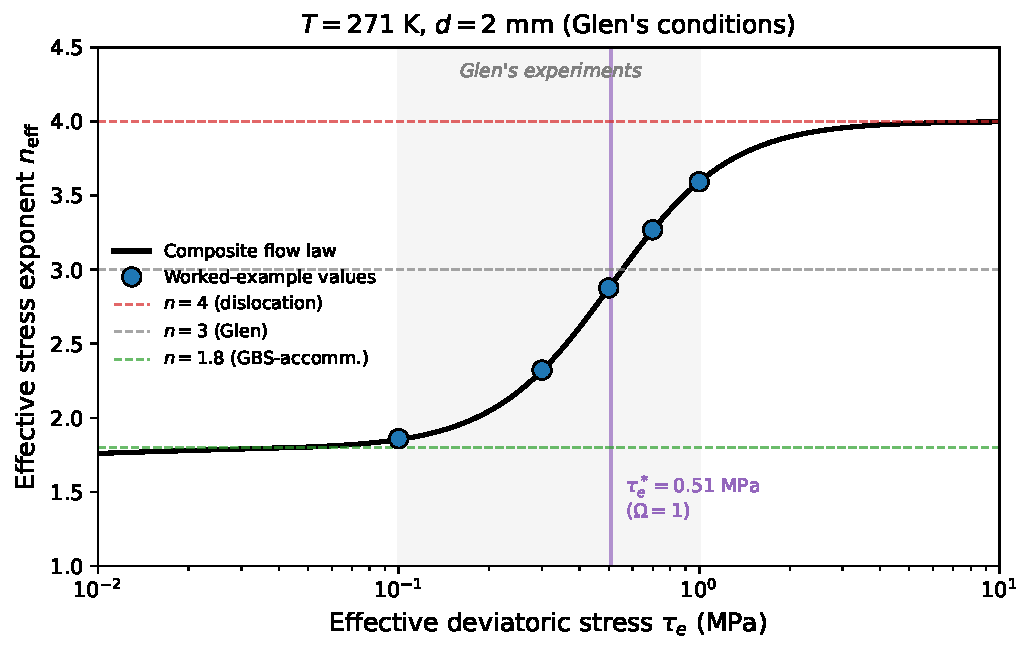
\includegraphics[width=0.75\textwidth]{figures/fig06_n_eff_glen_conditions.pdf}
  \caption{Effective stress exponent $n_{\text{eff}}$ as a function of stress at Glen's experimental conditions ($T = 271$~K, $d = 2$~mm).  The five points correspond to the values computed in the table above.  The crossover stress $\tau_e^* \approx 0.51$~MPa, where dislocation creep and GBS-accommodated basal slip contribute equally ($\Omega = 1$), is marked by a vertical line.  Glen's experimental stress range is shaded.}
  \label{fig:n_eff_example}
\end{figure}

\noindent Note that $\tau_e^*$ depends on temperature and grain size through equation~\eqref{eq:crossover_stress}.  Changing the grain size or temperature shifts the crossover and, with it, the apparent $n$ one would measure in any given experiment.  The specific numerical values in this example depend on the laboratory parameters of \cite{GoldsbyKohlstedt2001}; if the true exponents differ modestly from the lab values (e.g., $n \approx 3.5$ instead of 4.0 for dislocation creep), the crossover stress and the $n_{\text{eff}}$ values shift quantitatively but the qualitative picture---$n \approx 3$ as a transitional value between two mechanisms---is unchanged.

\subsection{Example 2: Slab on a Slope---How $n$ Changes the Velocity Prediction}
\label{sec:example_slab}

From the dynamics lectures, the surface velocity for a uniform slab of thickness $h$ on a slope $\alpha$ with no basal sliding ($u_b = 0$) is
\begin{equation}
  u_s = \frac{2A}{n+1}\left(\rho_i g \sin\alpha\right)^n h^{n+1}.
  \label{eq:us_slab}
\end{equation}
The basal shear stress is $\tau_b = \rho_i g h \sin\alpha$.  Because $u_s$ depends strongly on $n$ through both $\tau_b^{\,n}$ and $h^{n+1}$, the choice of creep exponent has large consequences for predicted velocities and their sensitivity to changes in glacier geometry.

\medskip
\noindent\textbf{Part 1: Two glaciological settings.}

\begin{center}
\begin{tabular}{lcccc}
\toprule
Setting & $h$ (m) & $\alpha$ & $T$ (K) & $\tau_b$ (MPa) \\
\midrule
A: Ice-sheet interior (e.g., East Antarctica) & 2500 & 0.1$^\circ$ & 243 & 0.039 \\
B: Steep outlet glacier (e.g., Alpine or Greenland) & 500 & 5$^\circ$ & 268 & 0.39 \\
\bottomrule
\end{tabular}
\end{center}

\noindent For Setting~A, the basal shear stress is $\tau_b = 917 \times 9.8 \times 2500 \times \sin(0.1^\circ) \approx 0.039$~MPa.  For Setting~B, $\tau_b = 917 \times 9.8 \times 500 \times \sin(5^\circ) \approx 0.39$~MPa.

\medskip
\noindent From Example~1, the composite flow law predicts $n_{\text{eff}} \approx 1.8$ in Setting~A (low stress, GBS dominates) and $n_{\text{eff}} \approx 2.7$--$3$ in Setting~B (near the crossover).  Glen's law with $n = 3$ is therefore a reasonable approximation for the outlet glacier but a poor one for the ice-sheet interior.

\medskip
\noindent\textbf{Part 2: Velocity sensitivity to thickness and slope.}  From equation~\eqref{eq:us_slab}, $u_s \propto h^{n+1}$ at fixed slope.  If the ice thickness increases by 10\% ($h \to 1.1\,h$), the velocity changes by a factor $1.1^{n+1}$:

\begin{center}
\begin{tabular}{ccc}
\toprule
$n$ & $1.1^{n+1}$ & Velocity increase \\
\midrule
1.8 & 1.31 & 31\% \\
3.0 & 1.46 & 46\% \\
4.0 & 1.61 & 61\% \\
\bottomrule
\end{tabular}
\end{center}

\noindent A 10\% thickness change produces a velocity increase that ranges from 31\% to 61\% depending on $n$---a factor of two in the \textit{sensitivity}, not just the velocity itself.

\medskip
\noindent Similarly, $u_s \propto (\sin\alpha)^n$ at fixed thickness.  Doubling the surface slope gives:

\begin{center}
\begin{tabular}{cc}
\toprule
$n$ & $2^n$ (velocity factor) \\
\midrule
1.8 & 3.5 \\
3.0 & 8.0 \\
4.0 & 16.0 \\
\bottomrule
\end{tabular}
\end{center}

\noindent The differences are dramatic: the velocity response to a steepening ranges from a factor of 3.5 to 16.  These results are summarized graphically in Figure~\ref{fig:velocity_sensitivity}.

\medskip
\noindent\textbf{Part 3: Velocity prediction error in the ice-sheet interior.}  The most consequential errors arise when Glen's law, calibrated at moderate stresses, is extrapolated to the low stresses of ice-sheet interiors (and high-stresses in fast-flowing regions).  Suppose Glen's law is calibrated to match observed strain rates at a reference stress $\tau_{\text{ref}} = 0.3$~MPa.  The predicted surface velocity at a different stress $\tau_b$ relative to the composite-law prediction scales as
\begin{equation}
  \frac{u_s^{\text{Glen}}}{u_s^{\text{composite}}} = \frac{n_{\text{eff}} + 1}{n_{\text{Glen}} + 1}\left(\frac{\tau_b}{\tau_{\text{ref}}}\right)^{n_{\text{Glen}} - n_{\text{eff}}},
  \label{eq:velocity_ratio}
\end{equation}
where $n_{\text{Glen}} = 3$ and $n_{\text{eff}}$ is the value predicted by the composite flow law.  For Setting~A ($\tau_b = 0.039$~MPa, $n_{\text{eff}} = 1.8$):
\begin{equation}
  \frac{u_s^{\text{Glen}}}{u_s^{\text{composite}}} = \frac{2.8}{4}\left(\frac{0.039}{0.3}\right)^{3 - 1.8} = 0.70 \times 0.13^{1.2} = 0.70 \times 0.086 \approx 0.060.
\end{equation}
Glen's law \textit{underpredicts} the deformation velocity in the ice-sheet interior by more than an order of magnitude.  This is because Glen's law ($n = 3$) applies too strong a stress dependence, making the strain rate drop off much faster at low stresses than the composite law ($n = 1.8$) predicts.  Figure~\ref{fig:velocity_ratio} shows how this ratio varies across a range of basal shear stresses.

\begin{figure}[ht]
  \centering
  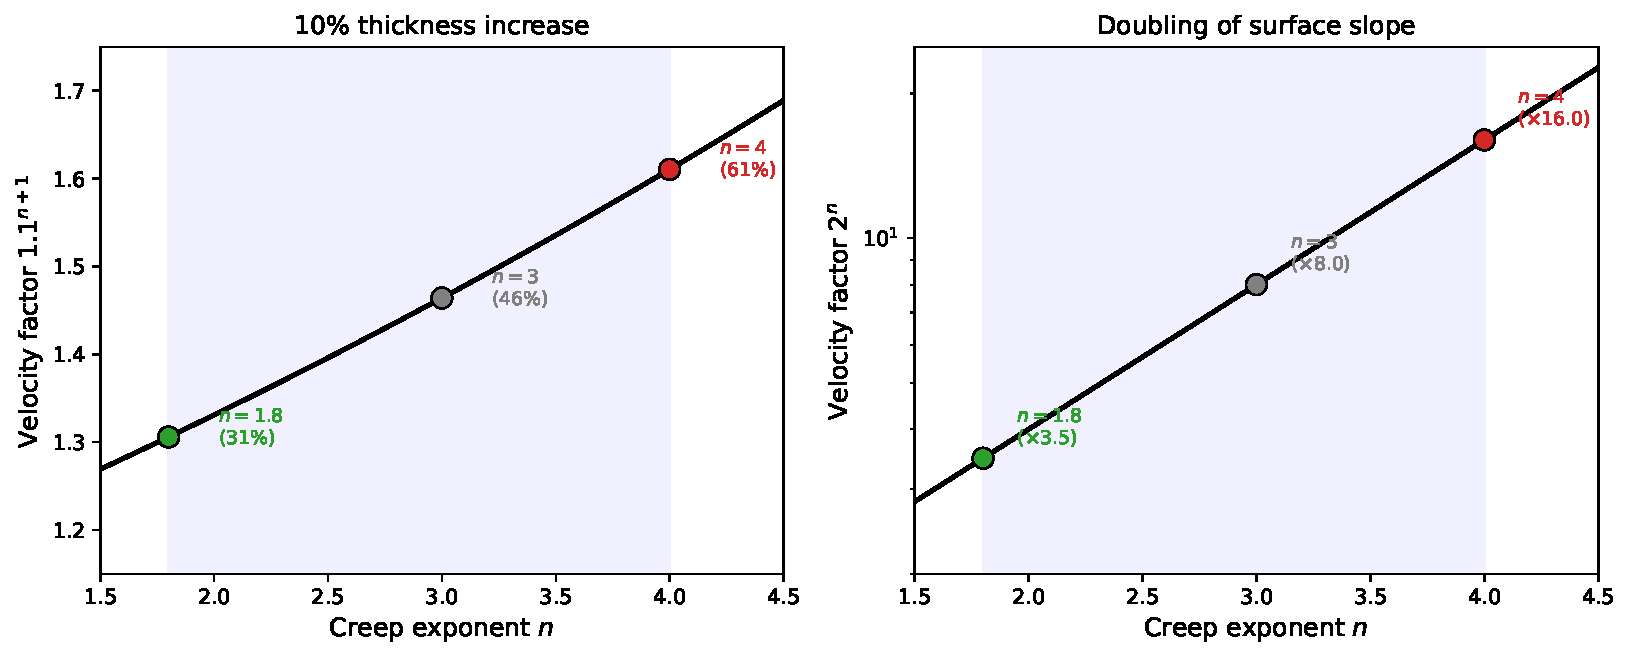
\includegraphics[width=0.85\textwidth]{figures/fig07_velocity_sensitivity.pdf}
  \caption{Sensitivity of surface velocity to the creep exponent $n$. \textbf{Left:} velocity change from a 10\% increase in thickness, $1.1^{n+1}$.  \textbf{Right:} velocity change from a doubling of surface slope, $2^n$.  Points mark $n = 1.8$, 3, and 4.  The shaded region spans the range of $n_{\text{eff}}$ predicted by the composite flow law.}
  \label{fig:velocity_sensitivity}
\end{figure}

\begin{figure}[ht]
  \centering
  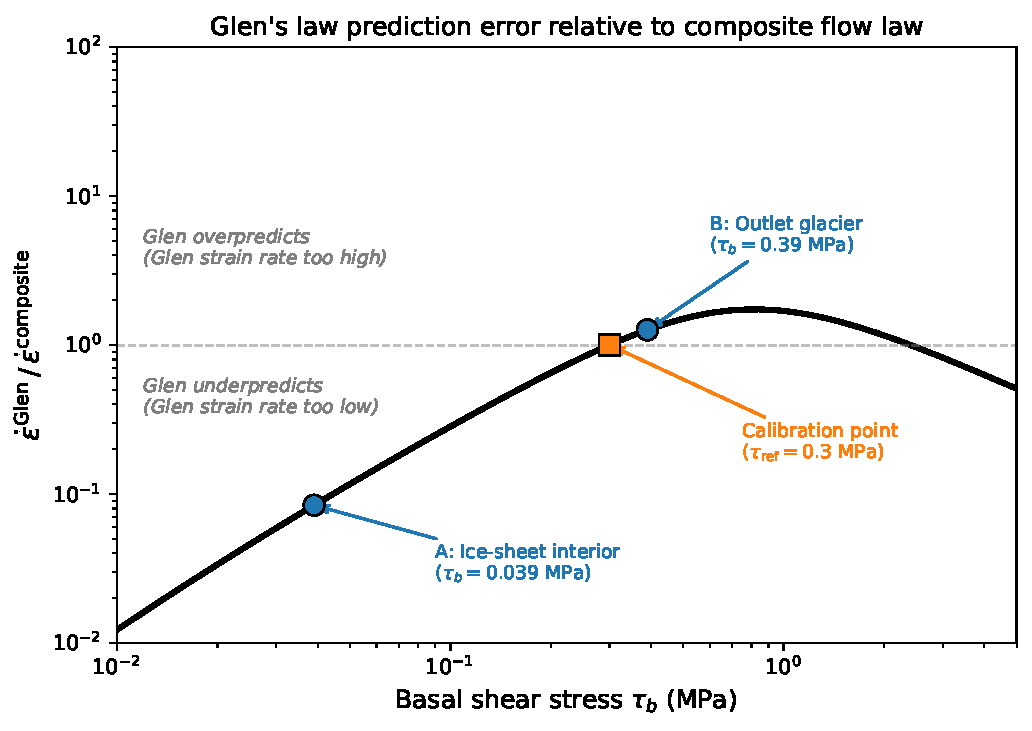
\includegraphics[width=0.75\textwidth]{figures/fig08_velocity_ratio.pdf}
  \caption{Ratio of surface velocity predicted by Glen's law ($n = 3$) to the composite flow law as a function of basal shear stress, assuming both laws are calibrated to give the same strain rate at $\tau_{\text{ref}} = 0.3$~MPa.  At low stresses (ice-sheet interiors), Glen's law underpredicts velocities by more than an order of magnitude because its $n = 3$ exponent makes the strain rate fall off too steeply.  At high stresses (shear margins, grounding lines), Glen's law underpredicts because the true exponent is closer to 4.  The two glaciological settings from this example are marked.}
  \label{fig:velocity_ratio}
\end{figure}

\noindent This result provides the physical basis for the modeling studies cited in the preceding section: the choice of $n$ is a first-order control on ice-sheet velocity predictions and, through them, on projections of sea-level rise.  When models are tuned to match present-day observations by adjusting $A$, the error in $n$ is absorbed---but it re-emerges as soon as the model is used to predict flow under different conditions (e.g., thinner ice, steeper slopes, warmer temperatures).  The specific factor of $\sim$18 computed above depends on the laboratory values of $n$; the direction and order-of-magnitude of the bias are robust to plausible variations in the exponents.

\subsection{Example 3: The Crossover Stress as a Stress Attractor}
\label{sec:example_attractor}

In \S\ref{sec:mechanism_maps} we noted that the crossover between GBS-accommodated basal slip and dislocation creep occurs at stresses of order $\sim$0.1~MPa---the same stress scale typical of glaciers and ice sheets.  This coincidence reflects a feedback between the creep mechanism, the effective viscosity, and the glacier's geometry.  Here we make this argument quantitative.

\medskip
\noindent\textbf{Part 1: Steady-state flux balance.}  Consider a uniform slab of ice on a slope $\alpha$ in steady state with no basal sliding.  The depth-integrated ice flux per unit width must balance the upstream accumulation:
\begin{equation}
  q = \dot{b}\,L,
\end{equation}
where $\dot{b}$ is the net accumulation rate and $L$ is the distance from the ice divide.  For a power-law rheology $\dot{\varepsilon}_e = A\,\tau_e^n$, the flux is (from the dynamics lectures)
\begin{equation}
  q = \frac{2A}{n+2}\left(\rho_i g \sin\alpha\right)^n h^{n+2}.
  \label{eq:flux_slab}
\end{equation}
The driving stress for the slab is $\tau_d = \rho_i g h \sin\alpha$ (which, in this geometry, equals the basal shear stress $\tau_b$).  Substituting $h = \tau_d / (\rho_i g \sin\alpha)$ into equation~\eqref{eq:flux_slab} gives $q \propto \tau_d^{n+2}$ at fixed slope: the flux is a steep power of the driving stress.

\medskip
\noindent\textbf{Part 2: How flux responds to stress.}  From equation~\eqref{eq:flux_slab}, $q \propto \tau_d^{n+2}$ at fixed slope.  The more nonlinear the rheology, the more sensitively the flux responds to stress:

\begin{center}
\begin{tabular}{ccc}
\toprule
$n$ & $q \propto \tau_d^{n+2}$ & $\tau_d \propto q^{1/(n+2)}$ \\
\midrule
1.8 & $\tau_d^{3.8}$ & $q^{0.26}$ \\
3.0 & $\tau_d^{5}$ & $q^{0.20}$ \\
4.0 & $\tau_d^{6}$ & $q^{0.17}$ \\
\bottomrule
\end{tabular}
\end{center}

\noindent Reading the table from left to right: at higher $n$, the flux increases more steeply with stress, which means that a glacier with higher $n$ needs only a small increase in driving stress to evacuate a much larger flux.  Equivalently (right column), the driving stress required to carry a given flux is a weaker function of $q$ at higher $n$.  A tenfold increase in $q$ requires the driving stress to increase by a factor of $10^{0.26} = 1.8$ in the GBS regime ($n = 1.8$), but only $10^{0.17} = 1.5$ in the dislocation creep regime ($n = 4$).

\medskip
\noindent\textbf{Part 3: The feedback.}  The composite flow law transitions from $n_{\text{eff}} \approx 1.8$ below the crossover stress to $n_{\text{eff}} \approx 4$ above it.  From the $q$--$\tau_d$ scaling in Part~2, this transition has a direct consequence for the glacier's stress state:

\begin{itemize}
  \item \textbf{Below the crossover} ($\tau_d < \tau_e^*$): the ice is in the GBS regime, with relatively high effective viscosity (weakly shear-thinning, $n = 1.8$).  The glacier can sustain a thick column.  As accumulation builds the ice up, thickness increases, driving the stress upward toward the crossover.  The stress responds to forcing as $\tau_d \propto q^{0.26}$.
  \item \textbf{Above the crossover} ($\tau_d > \tau_e^*$): the ice transitions into the dislocation creep regime, where the viscosity drops rapidly (strongly shear-thinning, $n = 4$).  The glacier flows fast and thins, reducing the stress.  The stress responds to forcing as $\tau_d \propto q^{0.17}$---the stress is less responsive, effectively ``capped'' by the strong shear thinning.
\end{itemize}

\noindent The net effect is a negative feedback that drives the stress toward the crossover.  Below it, stress rises relatively quickly with forcing; above it, the sensitivity drops and stresses plateau.  The crossover stress $\tau_e^*$---set entirely by the material properties of ice (the prefactors $A_0$, stress exponents $n$, and activation energies $Q$ of the competing mechanisms)---therefore acts as an attractor for the stress state of the glacier.

\medskip
\noindent\textbf{Part 4: Numerical demonstration.}  Figure~\ref{fig:stress_attractor} shows the steady-state basal shear stress as a function of specific flux $q$, computed numerically from the composite flow law for three surface slopes.  At each slope, the stress tracks the GBS power law at low fluxes and the dislocation creep power law at high fluxes, with a transition near the crossover stress $\tau_e^*$.  The stress varies by less than two orders of magnitude across six orders of magnitude of flux---and the crossover stress sits in the middle of the glaciologically relevant range.

\begin{figure}[ht]
  \centering
  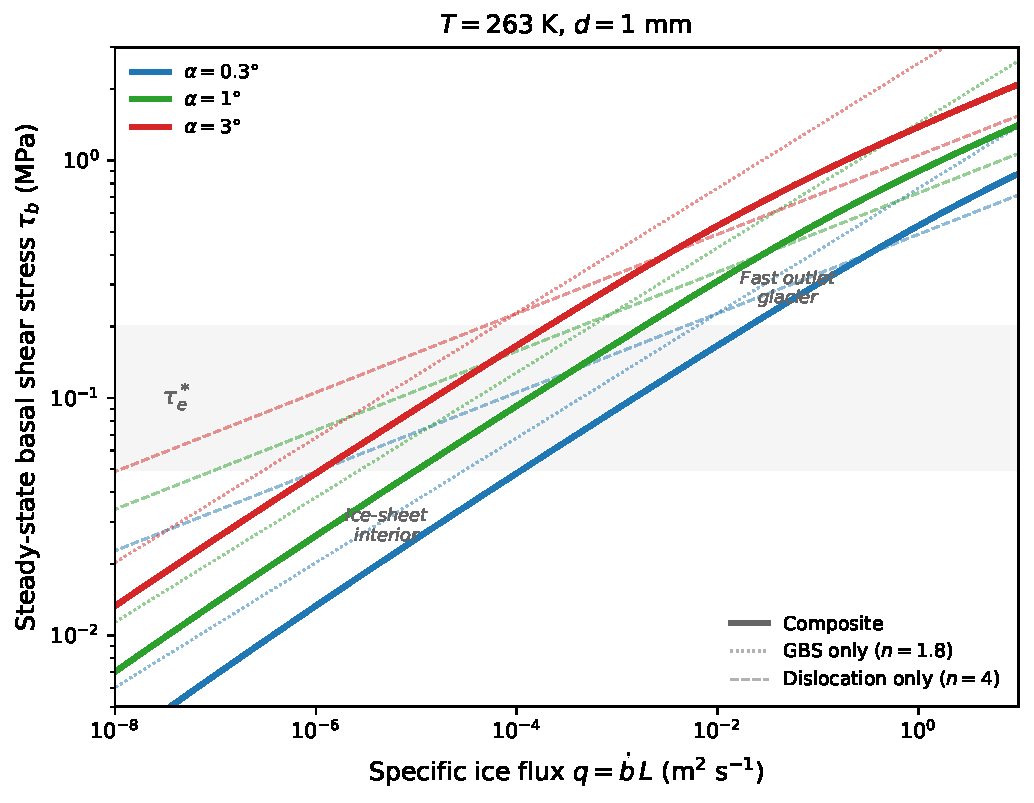
\includegraphics[width=0.75\textwidth]{figures/fig09_stress_attractor.pdf}
  \caption{Steady-state basal shear stress as a function of specific ice flux $q = \dot{b}\,L$ for three surface slopes, computed using the composite flow law ($T = 263$~K, $d = 1$~mm).  Thin lines show the predictions from the GBS mechanism alone ($n = 1.8$; steeper slope in $\log$-$\log$ space) and dislocation creep alone ($n = 4$; shallower slope).  The composite law (thick lines) transitions from GBS-dominated behavior at low fluxes to dislocation-dominated behavior at high fluxes.  The transition occurs near the crossover stress $\tau_e^* \approx 0.1$~MPa (horizontal band), which coincides with the typical stress scale of glaciers.  Specific fluxes representative of an ice-sheet divide region and a fast outlet glacier are marked for reference.}
  \label{fig:stress_attractor}
\end{figure}

\noindent The crossover stress is determined by the material properties of ice---not by the geometry or climate of any particular glacier.  The fact that glaciers on Earth, across a wide range of sizes, slopes, and accumulation rates, tend to have stresses of order $\sim$0.1~MPa is consistent with this rheological feedback.  The ice adjusts its geometry---and thus its stress---to sit near the boundary between the two dominant creep mechanisms.

\subsection{Example 4: Implications for Marine Ice Sheet Stability}
\label{sec:example_misi}

The value of $n$ also has qualitative consequences for our assessment of marine ice sheet stability.  Marine ice sheets---ice sheets whose beds lie below sea level---are thought to be vulnerable to a buoyancy-driven positive feedback known as the \textbf{marine ice sheet instability} (MISI) when the bed deepens toward the ice-sheet interior (a retrograde bed slope) \cite{Schoof2007}.  MISI has been invoked as a mechanism for the rapid retreat of the West Antarctic Ice Sheet and is a major source of uncertainty in sea-level projections.

\medskip
\noindent\textbf{The Schoof (2007) grounding line flux.}  \cite{Schoof2007} showed, using a boundary layer analysis of the shallow-shelf equations, that the ice flux at the grounding line (the boundary between grounded and floating ice) depends on the ice thickness there as a steep power law:
\begin{equation}
  q_g = \Lambda(A, n, C)\;\; h_g^{\,\gamma(n,m)}, \qquad \gamma(n,m) = \frac{mn+3m+1}{m+1},
  \label{eq:schoof_flux}
\end{equation}
where $h_g$ is the ice thickness at the grounding line (set by a flotation condition), $C$ is a basal sliding coefficient, $\Lambda$ is a prefactor that depends on $A$, $n$, $C$, and physical constants, and $m$ is the exponent in the Weertman sliding law $u_b = C\,\tau_b^m$ (the same convention used in the dynamics lectures).  A common assumption is $m = n$.  The exponent $\gamma$ increases with $n$; in the perfectly plastic limit ($m \to \infty$), $\gamma \to n + 3$:

\begin{center}
\begin{tabular}{ccc}
\toprule
$n$ & $\gamma(n,\,m=n)$ & $\gamma(n,\,m\to\infty)$ \\
\midrule
1.8 & 3.4 & 4.8 \\
3.0 & 4.75 & 6.0 \\
4.0 & 5.8 & 7.0 \\
\bottomrule
\end{tabular}
\end{center}

\noindent Higher $n$ means the grounding line flux is more sensitive to the local ice thickness, and thus to changes in bed depth.

\medskip
\noindent\textbf{Steady states and stability.}  In steady state, the grounding line flux must balance the upstream accumulation: $q_g(x_g) = \dot{b}\,x_g$, where $x_g$ is the grounding line position.  This condition is satisfied where the $q_g(x_g)$ curve intersects the accumulation line $\dot{b}\,x_g$ (Figure~\ref{fig:misi}).  On a prograde bed (deepening seaward), these intersections are stable: a small perturbation in grounding line position produces a restoring flux imbalance.  On a retrograde bed, however, the intersection is unstable: retreat into deeper water increases $h_g$, which increases $q_g$, which drives further retreat---a positive feedback.

\medskip
\noindent\textbf{How $n$ controls stability.}  Changing $n$ changes both the exponent $\gamma$ in equation~\eqref{eq:schoof_flux} and the prefactor $\Lambda$ (through its dependence on $A$).  When $n$ and $A$ are coupled through the composite flow law, the combined effect can qualitatively change the stability picture.  Figure~\ref{fig:misi} illustrates this for an idealized bed geometry with a retrograde section.  The three flux curves---computed for $n = 1.8$, 3, and 4 with corresponding $A$ values from the composite flow law---intersect the accumulation line at different positions and with different stability properties.  The number and location of unstable steady states on the retrograde section depend on $n$: some values of $n$ produce MISI for this bed geometry while others do not.  \cite{RanganathanMinchew2024} showed that this sensitivity extends to realistic ice-sheet configurations, with the potential for MISI appearing or disappearing depending on the assumed $(n, A)$ pair.

\begin{figure}[ht]
  \centering
  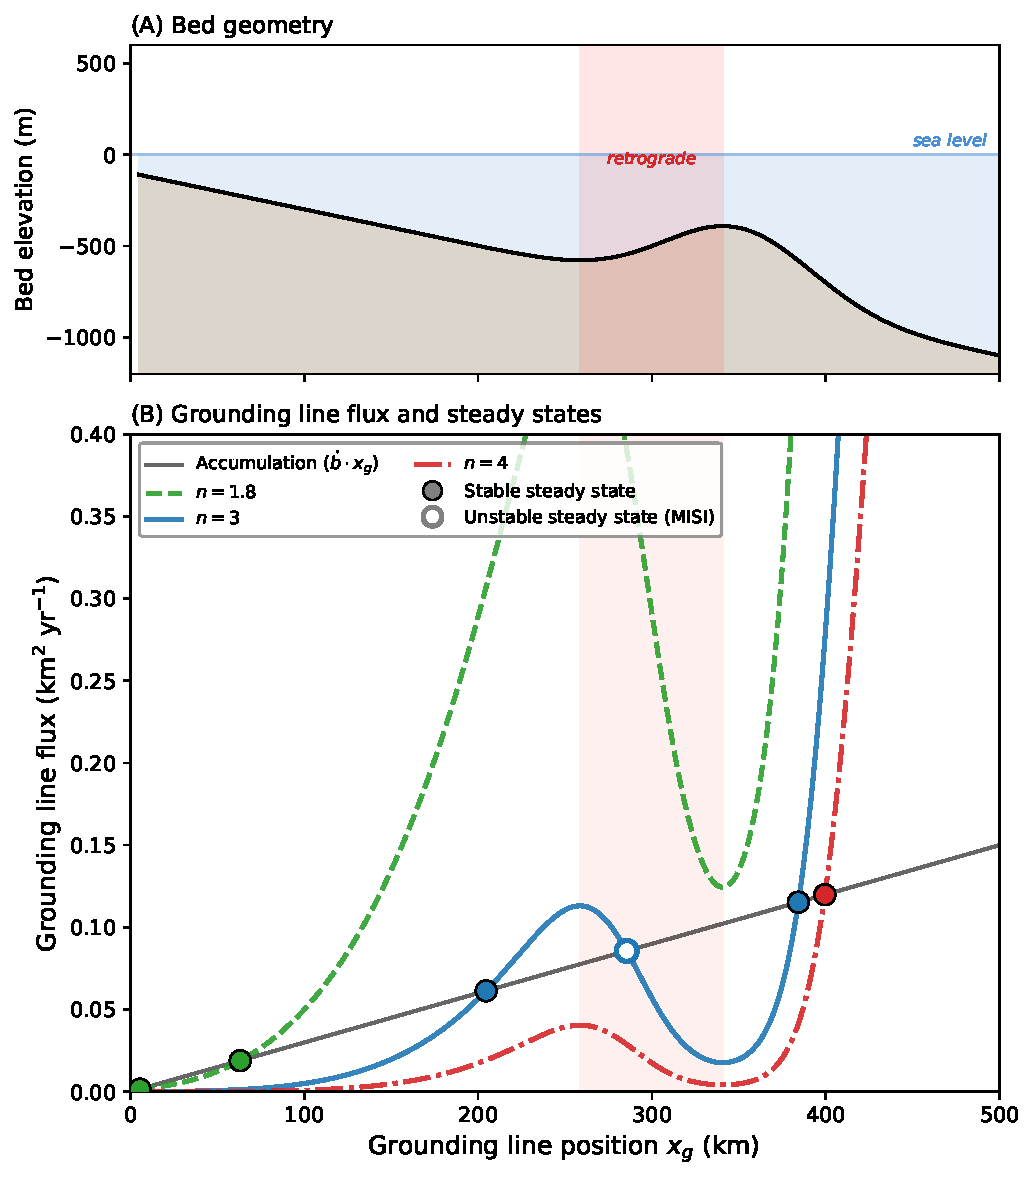
\includegraphics[width=0.8\textwidth]{figures/fig10_misi_stability.pdf}
  \caption{\textbf{(A)} Idealized bed geometry with a retrograde section (shaded).  \textbf{(B)} Grounding line flux $q_g(x_g)$ for three values of $n$ with corresponding $A$ values from the composite flow law, plotted against the accumulation line $\dot{b}\,x_g$.  Intersections are steady-state grounding line positions; filled circles are stable, open circles are unstable (MISI).  The number and location of steady states---and whether any are unstable---depend on the assumed $n$ and $A$.  Following the analysis of \cite{RanganathanMinchew2024}, adapted from \cite{Schoof2007}.}
  \label{fig:misi}
\end{figure}

\noindent The conclusion is that our assessment of whether a marine ice sheet is vulnerable to unstable retreat depends on the assumed rheology.  Different values of $n$---each with the corresponding $A$ from the composite flow law---produce different stability landscapes for the same bed geometry and accumulation rate.  Since the composite flow law predicts that the effective $n$ varies spatially across an ice sheet (\S\ref{sec:composite}), the stability of any given grounding line depends not just on the bed geometry and climate forcing, but on the local rheological regime---which is itself determined by the stress, temperature, and grain size.

\medskip
\noindent\textbf{An open question.}  The Schoof formulation separates the grounding line flux into a prefactor $\Lambda$ and a thickness-dependent term $h_g^{\,\gamma}$, treating $A$, $n$, $C$, and $m$ as independent constants.  With the composite flow law, this separation breaks down: $A$ and $n$ depend on the effective stress, and the effective stress at the grounding line depends on the driving stress, which is set by the combined effects of the ice viscosity, the sliding law, and the accumulation rate.  The prefactor $\Lambda$ is therefore not independent of the glacier's state---it is coupled to the same stress field that determines $n_{\text{eff}}$.

\medskip
\noindent This brings us back to the stress-attractor argument of Example~3.  If the composite flow law drives glacier stresses toward the crossover between GBS and dislocation creep (\S\ref{sec:example_attractor}), then the effective $n$ and $A$ at the grounding line are not free parameters but are constrained by the same rheological feedback that controls the stress state of the ice sheet.  Whether this feedback always produces conditions for MISI, never does, or does so only under specific combinations of bed geometry and accumulation remains an open question---and one with direct consequences for projections of marine ice sheet retreat and sea-level rise.

\clearpage
%===================================================================
% Reading
%===================================================================
\section*{Reading}

Cuffey \& Paterson, \textit{Physics of Glaciers}, 4th ed.:
\begin{itemize}
  \item Section 3.4: The flow law---overview and experimental basis
  \item Section 3.4.4: Creep mechanisms and the stress exponent
  \item Section 3.4.6: Temperature dependence and the rate factor
\end{itemize}

%===================================================================
% Bibliography
%===================================================================
\bibliographystyle{plainnat}
\bibliography{../references}

\end{document}
